\chapter{Experiments: Optomechanics}
% References are needed for historical context, technical claims, and specific data.
% Suggested [?] placements below:

This chapter will cover the experimental methods used in the development of optomechanical three-mirror cavity systems, focusing on the design, fabrication, and characterization of mechanical resonators within optical cavities. The methods are designed to enhance the sensitivity of measurements in quantum optics and optomechanics.
\minitoc
\newpage 

Over the past two decades, optomechanical systems have greatly benefited from advancements in optical coating technologies, enabling the realization of high-finesse cavities ($\mathcal{F}>10^5$)\cite{coating_review}. Simultaneously, progresses in micro/nanofabrication allowed the making of mechanical structures with high $Q$ factors ($>10^6$)\cite{nanofab_review}. Despite these achievements, a significant challenge remained: fabricating mechanical elements that possess both high $Q$ and high reflectivity, as optical, mechanical and thermal effects often degrade system performance and hinder ultra-sensitive measurements\cite{optomech_challenges}.
\section{System Description and Setup}

\subsection{Previous LKB work and Motivation}

Previous optomechanics experiments at LKB have primarily utilized Fabry--Pérot cavities with two mirrors, where the end mirror of the cavity was typically a HR mirror deposited on top of a mechanical structure featuring a mechanical mode of interest~\cite{}. 
\begin{itemize}
\item Over Aurélien's and Leonard's PhD works, the group in collaboration with ONERA developed a platform based on a $1$-mm-thick quartz micropillar with an effective mass of $33~\mu$g. The structure supports a fundamental compression mode oscillating at $3.6$~MHz, with a mode shape as shown in Fig.~\ref{fig:micropillar_mode}. Using a dry-film photoresist technique, a $100~\mu$m diameter high-reflectivity mirror was deposited on one end of the pillar. Careful design of the suspension has yielded mechanical quality factors up to $3\times 10^{6}$ at room temperature and up to $7\times 10^{7}$ below 1~K. When integrated into a $50~\mu$m-long Fabry--Pérot cavity with a custom-fabricated coupling mirror, finesses exceeding $10^{5}$ were achieved. Importantly, this compact cavity remains robust against vibrations of the dilution refrigerator and maintains alignment during cooldown, thereby providing a stable platform to study optomechanical effects in the intermediate mass regime. \color{red} limitations and why it didnt work \color{black}


\item Then over Rémi's and Michael's PhD, another resonator was developed in collaboration with Francesco Marin’s team, based on a suspended silicon disk. The device operates in a balanced mode, where the central disk vibrates in opposition to four surrounding counterweights. By adjusting the geometry, the resonance frequency was increased to $280$~kHz, corresponding to an effective mass of about $110~\mu$g, bringing the system closer to the micropillar parameters. A HR mirror was then deposited on top using the same technique as the micropillar. Finesse of about $\sim 50 000$ were then reached. At cryogenic temperature, optimized designs reached mechanical quality factors on the order of $1.2 \times 10^{6}$.\color{red} limitations and why it didnt work \color{black}

\end{itemize}

Although the systems ended up being limited by various factors mentioned above (optical, mechanical and thermal effects)~\cite{}, the parts designed over the years did feature a high level of passive stability as well as good thermalization properties.  A pivotal solution, introduced by Regal, Kimble, Harris, and collaborators\cite{Regal2008,Harris2008}, was to decouple these requirements by embedding a high-$Q$ mechanical resonator within a high-finesse optical cavity, using the optical field to probe and control the resonator’s dynamics.

\subsection{Specifications and Design}
It was then decided to build on this design and extend it to a three-mirror cavity in a MATE configuration to benefit from this large linear coupling range as detailed in the previous chapter. That is the work Michael and myself undertook during my M2 internship and the first year of my PhD.
This new three mirror cavity then needed to fulfill various requirements: 
\begin{itemize}
    \item \textbf{High Finesse}: input and back mirrors should both have high reflectivities, with low extra losses such as scattering, absorption, etc ...\cite{AmatoPhD}
    \item \textbf{High $Q$ factor}: the middle mirror i.e. the mechanical resonator, should feature a high $Q$ factor, ideally above $10^6$, in order to ensure a good sensitivity to radiation pressure forces\cite{SiN_review}
    \item \textbf{Optical alignement}: the cavity should be designed to allow for easy optical alignment, with the ability to mode match the setup fairly easily.
    \item \textbf{Dynamical range}: both input and output mirrors should be mounted on piezoelectric actuators, allowing for a dynamic range of at least few microns to scan few FSRs. The piezo actuators should also be able to provide a good bandwidth, ideally above 100 kHz, as well as a sub-nanometer resolution to ensure a good control of the cavity length\cite{piezo_review}.
    \item \textbf{Compactness \& Stability }: the entire assembly should be compact, with a high level of passive stability, yet without mechanically low pass filtering the piezo actuators motion during the locking. 
    \item \textbf{Vacuum and Cryogenic compatibility}: the cavity should be vacuum compatible, and the mirrors should be thermally anchored to the vacuum chamber in order to ensure a good thermalization of the system. Same holds for the cryogenic compatibility, although no test could be performed during this thesis. The cavity was nonetheless designed to be compatible with cryogenic operation.
\end{itemize}
\subsubsection{High Finesse}

Low loss mirrors were produced by \textbf{Jérôme~DEGALLAIX} and \textbf{David~HOFMAN} at the
\textit{Laboratoire des Matériaux Avancés} (LMA, Lyon) using
ion-beam-sputtered (IBS) Bragg stacks made of $\mathrm{Ta_2O_5}$ (high index,
$n\!\approx\!2.09$) and $\mathrm{SiO_2}$ (low index, $n\!\approx\!1.46$)\cite{AmatoPhD,LMA_IBS}. \\
The coatings were deposited in the LMA's \textit{Veeco SPECTOR} chambers and subsequently annealed at 500°C for 10 hours to minimise both optical (absorption) and mechanical losses, following the recipe of Amato \textit{et~al.}\,\cite{AmatoPhD}.
\footnote{Identical optics are used for the Advanced LIGO, Advanced Virgo
and KAGRA interferometers\cite{LIGO_optics}.}.\\

We supplied the LMA with a batch of substrates with various radii of curvature to explore different cavity geometries:
\begin{itemize}
  \item \textbf{Plane substrates:} Laseroptik S--00798
  \item \textbf{Plano-concave substrates:}
    \begin{itemize}
        \item Laseroptik S--00128 ($R = 20$ mm)
        \item Laseroptik S--00127 ($R = 15$ mm)
        \item Laseroptik S--00126 ($R = 10$ mm)
    \end{itemize}
\end{itemize}

All optics feature
\begin{itemize}
  \item \textbf{Back‐side AR:} $R \lesssim 100\,$ppm. This is not critical for the cavity performance since the back side is not actually contributing to the finesse, but it is important to avoid parasitic reflections in the setup.
  \item \textbf{Front‐side HR:}
    \begin{itemize}
        \item[] $T \sim 20 \pm 4\,$ppm on the plane mirrors,
        \item[] $T \sim 50 \pm 10\,$ppm and $100 \pm 10\,$ppm on the
                concave mirrors, respectively,
    \end{itemize}
  \item total round‐trip scatter\,+\,absorption
        $\lesssim 20\,$ppm, in agreement with the measurements reported (absoption $\sim$0.7ppm, scattering $\sim$10ppm)
        in Ref.\,\cite{AmatoPhD}.
\end{itemize}

The quarter‐wave design is centred at $\lambda = 1064$ nm for normal incidence.  After annealing, the measured mechanical loss angle of the $\mathrm{TiO_2\!:\!Ta_2O_5}/\mathrm{SiO_2}$ stack is $\phi < 4\times10^{-4}$ at 1 kHz  \color{red} link to mechanical damping needed \color{black}, supporting cavity finesses in the range $200\,000-500\,000$ before excess scatter or absorption dominates\cite{AmatoPhD}.

\subsubsection{High $Q$ factor}

The middle mirror is a commercially\,–\,available stoichiometric silicon-nitride
(Si$_3$N$_4$) membrane supplied by Norcada (NX10050AS)\cite{SiN_review,Norcada_datasheet}.
It consists of a $1\,\mathrm{mm}\times1\,\mathrm{mm}$, $50\,\mathrm{nm}$-thick
Si$_3$N$_4$ film suspended in a $10\,\mathrm{mm}\times10\,\mathrm{mm}$,
$200\,\mu\mathrm{m}$-thick silicon frame and is marketed specifically for
\emph{high-$Q$} resonator applications. Because stoichiometric LPCVD Si$_3$N$_4$ is under high intrinsic tensile
stress ($\sigma\!\approx\!0.9\;\mathrm{GPa}$), the square drum supports
MHz-frequency modes with exceptionally low mechanical loss\cite{SiN_review}.

\begin{itemize}
  \item \textbf{Room temperature.}  Measurements on nominally identical
        Norcada membranes report quality factors
        $Q \sim 5\times10^{6}$ at $\approx1\,\mathrm{MHz}$ in
        $<10^{-6}$ mbar vacuum \cite{SiN_review,Norcada_datasheet}.
  \item \textbf{Cryogenic operation.}  Cooling to $T \lesssim 300\,\mathrm{mK}$
        reduces internal friction by an order of magnitude, with
        $Q>10^{7}$ routinely observed \cite{SiN_cryogenic}.
\end{itemize}

On the basis of these results we set the following design targets:
\[
  Q_{\mathrm{RT}} \ge 5\times10^{6}, \qquad
  Q_{\mathrm{cryogenic}} \ge 1\times10^{7}.
\]
The membrane’s high stress, thin-film nature and dielectric composition make
it fully compatible with ultra-high-vacuum environments and repeated
cryogenic cycling, while introducing (a priori) negligible optical loss in the cavity.
These attributes ensure a robust, spectrally clean mechanical resonator for
advanced quantum-optomechanics experiments.

\subsubsection{Optical alignment}
The cavity is designed to be compatible with the Thorlabs cage system. The input mirror is mounted on a 3 axis cage mount, allowing for easy alignment of the input mirror with respect to the cavity optical axis. Both the resonator and the back mirror are embedded within a custom-made holder, which is itself integrated into the cage system. The relative tilt between the resonator and the back mirror is adjusted using a set of 3 screws with a very fine thread, allowing for a fine alignment of the parallelism of the back cavity. The alignment procedure is detailed in section~\ref{sec:alignment_procedure}.

\subsubsection{Dynamical range}

The input (front) mirror is glued to a PI \texttt{P-016.00H} ring-stack piezoelectric actuator using vacuum epoxy (Torr Seal). Driven from 0 to $+1000\,\mathrm{V}$ it provides a longitudinal stroke of $5\,\mu\text{m}$, a blocking force of $2.9\,\mathrm{kN}$, as well as an unloaded resonance of 144 kHz, making it suitable for fast, low-noise cavity-length control.

The end-mirror–membrane assembly is mounted on a flexure holder actuated by three \texttt{PD080.31} piezo chips arranged mechanically in series. Each chip yields $2\,\mu\text{m}$ of travel over a drive range of $-20$ to $+100\,\mathrm{V}$; the triple stack therefore supplies roughly $6\,\mu\text{m}$ of coarse tuning while preserving high stiffness and sub-microsecond response.

Combining the $5\,\mu\text{m}$ stroke of the front \texttt{P-016.00H} with the $6\,\mu\text{m}$ range of the rear triple stack provides an overall cavity-length adjustment of about $11\,\mu\text{m}$ — equivalent to more than 20 free spectral ranges — with sub-nanometre resolution when driven by low-noise high-voltage amplifiers.


\subsubsection{Compactness \& Stability}
The entire assembly is built as a cage system using standard Thorlabs cage parts, allowing for a compact and stable assembly\cite{Thorlabs_cage}. The cage system also allows for (relatively) easy alignment of the mirrors, as well as easy access to the piezo actuators.

\subsubsection{Vacuum and Cryogenic compatibility}
The back cavity composed of the back mirror and the middle mirror is embedded inside an Oxygen Free Copper (OFHC) assembly with a circular geometry, eventually mitigating for transverse misalignment issues when going to cryogenic temperatures, the constraints compensating themselves radially with respect to the symmetry axis of the cavity assembly\cite{OFHC_review}. Furthermore, the screws used to hold the assembly together are made of brass with a thermal expansion coefficient lower than that of the OFC, tightening up the cavity when reaching cryogenic temperatures.
Thorlabs cage parts are compatible with moderate vacuum operation down to $\sim 10^{-5} mbar$ if properly degreased and ultrasound cleant, but a custom cryocompatible system to hold the input mirror would be needed for operation at cryogenic temperatures. \\


\begin{figure}[H]
    \centering  
    \includegraphics[width=\textwidth]{./chap5/fig/schéma_cavity.pdf}
    \caption{Cavity design and assembly. (a) The figure shows the overall assembly of the MATE system from various views, highlighting the integration of the high-finesse mirrors, the membrane resonator embedded inside the back cavity copper assembly held to the input mirror Thorlabs holder through a cage system.(b) The exploded view details the arrangement of the mechanical and optical components, illustrating the modular design that facilitates alignment, stability, and compatibility with vacuum environments.}
    \label{fig:cad_cavity}
\end{figure}


The initial design of the cavity was made using Autodesk Fusion 360, allowing for a detailed 3D model of the entire assembly, including the piezo actuators, the mirrors and the cage system. The design was then exported to a STEP file format, which was used to manufacture the parts using a 3 axis CNC milling machine and a digital lathe. The pieces were machined by \textbf{Carounagarane~DORE} and \textbf{Gael~COUPIN} at the LKB mechanical workshop with 100$\mu$m tolerance. A detailed view of the cavity design and assembly is shown in Fig.~\ref{fig:cad_cavity}.

\subsection{Flexure Actuation}

One specificity of the MATE system is that the back cavity is significantly shorter than the front cavity, which would require high precision in both the machining of the copper pieces and the positioning of the resonator. In our case, we aim at a centimetric cavity which would require to position the membrane at roughly hundreds of microns from the back mirror, and parallel to the back mirror. Moving the membrane independently from the back mirror while maintaining a controllable tilt between both planes is therefore complicated. \\


A smart workaround was introduced by Jack Sankey and its group \cite{Sankey2010}, where the authors introduced a flexure-tuned MATE system. The key innovation lies in actuating the membrane position by flexing its supporting silicon frame rather than translating the entire mount. This is done by mounting the back cavity in a semi-monolitic fashion, and 'locking' the silicon frame of the membrane using three screws with a fine thread, allowing for a fine adjustment of the angle of the membrane plane with respect to the back mirror plane. The piezos pushing on the back of the assembly then force the silicon frame constrained by the screws to bend, thus displacing the membrane with respect to the back mirror, as shown in Fig.~\ref{fig:flexure tune}. 
This approach preserves the cavity alignment while enabling continuous and wide-range tuning of both the membrane displacement and tilt. 


\begin{figure}[H]
    \centering  
    \includegraphics[width=\textwidth]{./chap5/fig/flexure tune.pdf}
    \caption{Cavity design and assembly. (a) In this configuration (no voltage applied to the piezos), the screws are used to align the membrane plane with respect to the back mirror plane, ensuring a good parallelism between both planes. (b) Flexure tuning of the membrane position. When a voltage is aplied to the piezos, they push on the back of the assembly, forcing the silicon frame to bend, thus displacing the membrane with respect to the back mirror. The two dashed lines show the initial positions of the back mirror and the membrane. This push shortens the overall cavity length (i.e. increasing the overall system's frequency), as well as the relative distance between the mirror and the membrane (i.e. changing the optomechanical coupling). }
    \label{fig:flexure tune}
\end{figure}


\color{black}

\subsection{Experimental Setup}
The assembly is now to be integrated into the optical setup shown in Fig.~\ref{fig:optical layout}. The source laser is a 1064nm Nd:YAG laser (Coherent Mephisto). We did not require the full optical power delivered by the laser, so a short optical path not detailed here splits the laser in 3 arms to eventually fiber couple some laser power and bring it to other experiments that would need 1064nm laser light. \newline

\begin{figure}[h!]
    \centering  
    \includegraphics[width=\textwidth]{./chap5/fig/fig_lock_MATE.pdf}
    \caption{}
    \label{fig:optical layout}
\end{figure}
The optical path then consists of : 
\begin{itemize}
  \item a first half waveplate and a beam splitter to adjust the total power injected into the experimental setup,
  \item a fibered electro-optics phase modulator (EOM Photline NIR-MPX-LN-10) to generate sidebands for the PDH locking of the cavity. It is polarization matched by using a fibered polarization controller to avoid Residual Amplitude Modulation noise (RAM) at the output (three blue circles on the optical layout). 
  \item a fiber coupler to go from a guided optical mode to a free space optical mode, with a the coupler adjusted such that the outputted beam is collimated and has a waist of about 1mm,
  \item a quarter waveplate to compensate for ellipticity of the output beam polarization, then a half waveplate and a beam splitter to adjust the powers injected into the cavity path and the prospective LO path, respectively,
  \item on the cavity path, a faraday rotator to ensure the cavity reflected beam to be deflected to an output port and not back into the fiber 
  \item a lens to mode match the laser input mode to the cavity mode, with a focal length of 40 to 60mm depending on the input mirror radii of curvature. This lens is mounted on a x-y cage system translation mount, and is mounted inside the vacuum chamber that features AR coated windows to allow for optical access yet minimal parasite reflections.
  \item the cavity itself. 
  \item two photodiodes (Thorlabs ???) to detect the reflected beam and the transmitted beam, respectively, with 40mm focal length lenses to focus the beam onto the photodiodes. 
\end{itemize}

The optical path was designed to be as modular as possible, allowing for easy replacement of the components if needed, as well as additions of optical elements. For this reason, it features two fainted additional optical paths as seen on Fig.~\ref{fig:optical layout}, one for a prospective LO, and another to deflect the reflected beam to a Homodyne Detection setup using a flip mirror. Polarization optics would aslo need to be added on the Homodyne Detection path to mix the LO and the reflected beam, but this was not done during this thesis.

\subsection{Alignment Procedures}
The optical setup is now to be aligned as to ensure a good mode matching between the laser input mode and the cavity mode. The steps are as follows, and the associated diagrams are shown in Fig.~\ref{fig:tilt}:
\begin{itemize}
  \item \textbf{Step 1} (Fig.~\ref{fig:tilt}(a))\textbf{:} we position an iris diaphragm before our two injection mirrors mounted on ($\theta_x$,$\theta_y$) kinematic mounts. We then adjust the tilt of both mirrors i.e. \textit{beam-walking}, such that the reflected beam is centered on the iris diaphragm: this is done by maximising the reflected signal on the reflection photodiode. This ensure the beam reflected by the output mirror (HR mirror) is at normal incidence. In a second time we tune the plane of the resonator using the three screws of the assembly. We monitor the Fizeau fringes in transmission with a camera (Allied Vision Alvium), and adjust the tilt such that no fringes are to be seen. 
  \item \textbf{Step 2} (Fig.~\ref{fig:tilt}(b))\textbf{:} we then place the focusing lens in the optical path, and adjust its position such that we recover maximal power on the reflection photodiode. This lens is mounted on the (x-y) cage system translation mount, and positioned at a distance from the back mirror fixed by the cavity mode matching requirements (ref chap theory). The lens is then fixed in place using the cage system screws.
  \item \textbf{Step 3} (Fig.~\ref{fig:tilt}(c))\textbf{:} we add the input mirror on a ($\theta_x$,$\theta_y$) cage system mount, and adjust its position to get an input beam normal to the tangent of the concave mirror curvature. This is also done maximising the reflected power on the reflection photodiode. The mount (and thus the mirror) was also positioned at the appropriate distance from the back mirror to ensure optimal mode matching. 
  \item \textbf{Step 4} (Fig.~\ref{fig:tilt}(d))\textbf{:} We scan the cavity length using the piezo actuator mounted on the input mirror, and monitor the cavity resonances using both the reflected and transmitted photodiodes. We finally fine tune the mode match by \textit{beam-walking} the two injection mirrors. We can also play with the collimating lens at the fiber coupler (not shown on the diagram) as to fine tune for longitudinal mode matching. The cavity is now aligned and ready for operation.
  \end{itemize}

\begin{figure}[h!]
    \centering  
    \includegraphics[width=\textwidth]{./chap5/fig/tilt_alignementB.pdf}
    \caption{Set up alignment procedure. (a) to (d) show the steps to align the cavity with respect to the optical path (detailed in the main text). The (a.i) to (a.iv) show what is seen on the camera 4 four different tilt positions where (a.iv) displays a 'good' tilt alignement: no visible fringes except for the dim fringes of the camera setup. These dim fringes are present when the beam is a normal incidence with the back mirror (use of the iris) and are believed to be intereferences arising from reflections inside the camera objective as they are seen whatever the plane of focus is. }
    \label{fig:tilt}
\end{figure}
\section{Experimental Characterization}
\subsection{Cavity Characterization}
Once the cavity is aligned, we can scan the cavity length by driving the front mirror piezo with a triangular or a sine wave voltage. This signal is first amplified using a high voltage amplifier made by the LKB electronic workshop, which can deliver up to 1000V. The output impedance of the amplifier is a standard 50 Ohms, but the piezo in derivation at the end of the line with capacitance of about 15 nF low pass filters the signal at  $\sim$ 200 Hz. We can also modulated the back piezo actuators, in DC or AC, and a similar lowpass filtering occurs with a lower cutoff frequency $\sim$ 50Hz (3 piezo actuators in parallel with a capacitance of around 100 nF each). We call the input mirror piezo voltage $V_{\text{SW}}$ as it is used to scan the cavity length, and the back piezo voltage $V_{\text{DC}}$ as it is used to set the membrane position, and we model the these voltages as third order polynomials of the actual displacements $L-x$ and $x$ respectively. \\

We then monitor the cavity resonances using both the reflected and transmitted photodiodes and scanning the cavity over a large range, as to mode match the cavity to the TEM00 mode. By beam walking, we optimally mode match the cavity such that higher order modes vanish in the photodiode noise floor and the reflected and transmitted signals are maximised, we can then perform finer scans to characterize the cavity parameters.

Using the IR EOM as a frequency ruler, setting a reference between few MHz to $\sim$ 60 MHz (limited by the RedPitaya) we perform lorentzian fits of the three lorentzian dips, and compare the fitted positions. Two typical scans are shown in Fig.~\ref{fig:cavity_scan}, one large scan over few cavity FSRs, and a narrow one. \\ 

\noindent  \textbf{Finesse :} We can used three different methods to evalutate the finesse of the cavity. 
\begin{itemize}
  \item The first one would be to scan the cavity over few FSRs, and fit the lorentzian dips such that we can extract the ratio of their interspacings to their linewidths. This method is quite sensitive to the piezo nonlinearities, arising both from the system's transfer function and from the low pass filtering of the voltage ramp by the electronics. One can however used a sine ramp below the electronics cutoff frequency and calibrate the disaplcement owing to the fact that each resonance corresponds to a displacement of $\lambda/2$ (one FSR). 
  \item The second method would be to scan the cavity over a single resonance, and use the EOM sidebands as a frequency reference to extract the linewidth of the resonance. This method is less sensitive to piezo nonlinearities, assuming the piezo sweep is quasi linear over the resonance width. 
  \item The third method would be to scan the cavity rapidly and observe a cavity ringdown, and compare the heights of the first two rebounds in transmission to their temporal spacings. This method is less sensitive to piezo nonlinearities, but requires a fast photodiode. Additionally we can vary the piezo sweep frequency to scan for various sweep rates. 
\end{itemize}

Many trial and errors for such a MATE cavity were realised over this thesis, but the cleaner data were obtained with a cavity made of an input concave mirror of radius of curvature $R=20mm$ and transmittivity $t_1=100ppm$, a plane back mirror of $t_2=20ppm$ and a cavity length of $L=17mm$. Hence, the theoretical finesse would be $\sim 52400$. \\ 

\noindent \textbf{Empty cavity: }By using the second method for our finesse estimation, the empty cavity finesse was measured to be $\sim 28000$, such that we deduce total loss of $\Sigma T_i = 225 \pm 20$ppm  (including losses). The LMA did not provide us with specification sheets for the exact mirrors we used, but the uncertainty on the sum of the transmissions is estimated to be around 15ppm. In turn, we can estimate the excess cavity losses to be around $\gamma = 105ppm$. \color{red} errors \color{black} \\

\noindent \textbf{MATE cavity: }Once the membrane is inserted inside the cavity, both the resonant frequencies and the linewidths-finesse vary as a function of the membrane position $x$. Using our third order polynomials to model the piezos voltage seed to displacements transduction, we renormalize both the input mirror voltage sweep $V_{\text{SW}}$ and the back mirror voltage DC $V_{\text{DC}}$ to the cavity FSR and the nominal membrane displacement $x$ respectively. Knowing or laser wavelenth, this fit allows us to estimate the membrane reflectivity $|r_m|$ which is found to be 0.54. \color{red} link to expected value \color{black} \\ 

These fits then give us the total maps of available displacements $L-x$ and $x$ as a function of both $V_{\text{SW}}$ and $V_{\text{DC}}$, as shown in Fig.~\ref{fig:maps}. \\ 

\begin{figure}[h!]
    \centering  
    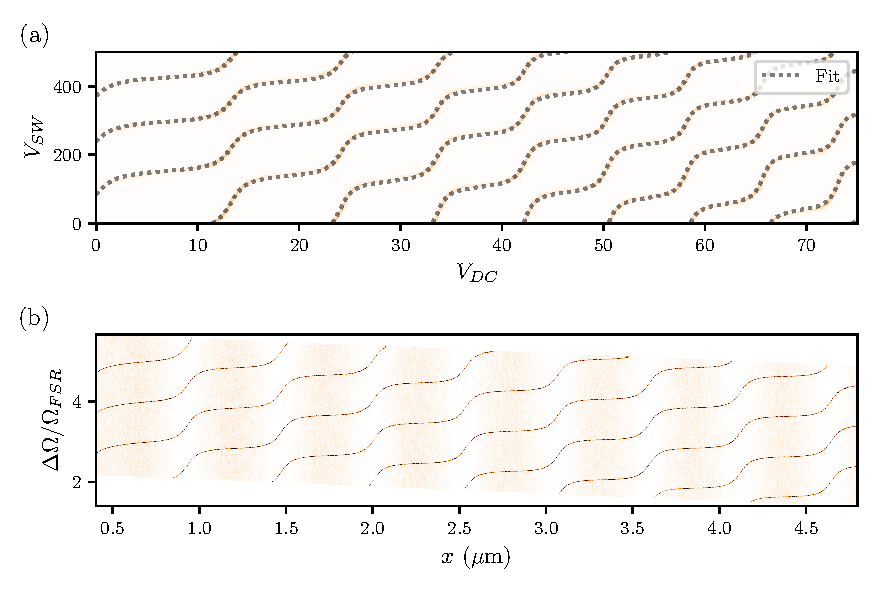
\includegraphics[width=\textwidth]{./chap5/fig/scansTot.pdf}
    \caption{ }
    \label{fig:tilt}
\end{figure}

\begin{figure}[h!]
    \centering  
    \includegraphics[width=\textwidth]{./chap5/fig/scancoupling.pdf}
    \caption{ }
    \label{fig:tilt}
\end{figure}

\begin{figure}[h!]
    \centering  
    \includegraphics[width=\textwidth]{./chap5/fig/scantrans.pdf}
    \caption{ }
    \label{fig:tilt}
\end{figure}

\noindent \textbf{Position dependent finesse: } We now record cavity scans at increasing values of $V_{DC}\propto P_3(x)$. The finesse oscillates between $\sim 6000$ and $\sim 20000$, which corresponds to total losses $\Sigma T_i$ between 300ppm and 1050ppm. This is significantly higher than the empty cavity losses, which indicates that the membrane introduces significant additional losses. 

Using the IR EOM as a frequency ruler, we can perform slow scans of the cavity length while monitoring the transmitted intensity. By carefully controlling the piezo voltage and using a lock-in amplifier to extract the signal, we can obtain high-resolution measurements of the cavity resonances. This technique allows us to probe the cavity modes with great precision and is particularly useful for characterizing the effects of the membrane on the cavity dynamics.
\subsection{Locking Techniques and Stability}
\subsection{Optical Ringdowns and Loss Measurements}
\subsection{Mechanical Resonator Characterization}
\subsection{Bistability}

\section{Design of an Optomechanical Fibered Cavity}
\subsection{Design considerations}

\vspace{-\baselineskip}

